%\documentclass[9pt]{beamer} 
\documentclass{beamer} 	%del imecc
\usepackage{beamerthemeshadow}
\usepackage{amsmath, amssymb, amsfonts, textcomp}
%=========================================================================================
\usepackage[brazilian]{babel}
% \usepackage[latin1]{inputenc}
\usepackage[utf8]{inputenc} % 
\usepackage{ragged2e}
\justifying
\setbeamertemplate{bibliography item}{[\theenumiv]}
\definecolor{airforceblue}{rgb}{0.36, 0.54, 0.66}
	%\definecolor{blue(ryb)}{rgb}{0.01, 0.28, 1.0}
\usetheme{Ilmenau}			% estilo y color de la presentacio
%\usetheme{JuanLesPins}		% estilo y color de la presentacio
\setbeamercolor{structure}{fg=airforceblue}
\mode<presentation>
\usepackage{times}
\usepackage[T1]{fontenc}	 %  
\usepackage{pgf, tikz}
\usetikzlibrary{arrows}
\usepackage{ stmaryrd }

%~~~~~~~~~~~~~~~~~~~~~~~~~~~
\usepackage{bbm}
\usepackage{eufrak}
\usepackage[mathscr]{euscript}
\usefonttheme{serif}
%~~~~~~~~~~~~~~~~~~~~~~~~~~~
% \pgfdeclareimage[height=1.0cm]{logo}{logounicamp}
\pgfdeclareimage[height=1.0cm]{encpos2020}{Figuras/encpos2020}
\logo{\pgfuseimage{encpos2020}}
% - - - - - - - - - - - - - - - - - - - - - - - - - - - - - - - - - - - - - - - - - - -
% figura 
\usepackage{subfig}
% \captionsetup[subfigure]{style=default, margin=0pt, parskip=0pt, hangindent=0pt, indention=0pt, singlelinecheck=true, labelformat=parens, labelsep=space}
% Caso queira guardar as figuras em uma pasta separada% - - - - - - - - - - - - - - - - - - - - 
% (descomente e) defina o caminho para o diretório:
%\graphicspath{{./figuras/}}

% Customizar as legendas de figuras e tabelas
\usepackage{caption}
\usepackage{empheq}

\newcommand{\vazio}{\emptyset}
\newcommand{\set}[1]{\left\{#1\right\}}

\begin{document}
%%TÍTULO-------------------------------------------
\author{Autor(es)}
\title{Título}
\institute{Universidade}
\titlegraphic{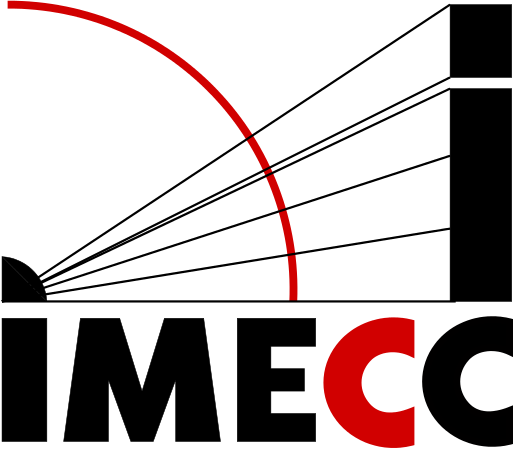
\includegraphics[width=1cm]{Figuras/imecc.png}~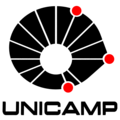
\includegraphics[width=1cm]{Figuras/logounicamp.png}}
\date{\today}

\frame{\maketitle}

\AtBeginSection[]
{  \begin{frame}<beamer>{Conteúdo}
    \tableofcontents[currentsection]
  \end{frame}}
%% - - - - - - - - - - - - - - - - - - - - - - - - - - - - - - - - - - - - - - - - - - -
% Conteudo do trabalho
%=======================================
\section{Introdução }
%===========================================
\begin{frame}{Introdução}  %
%===========================================
Bem Vindo(a)
 	
O Encontro Científico de Pós-Graduandos do IMECC (EnCPos) teve sua primeira edição no ano de 2004 e tem como intuito criar um ambiente que favoreça a interação entre os alunos de pós-graduação em Matemática, Matemática Aplicada e Estatística, além de propiciar uma oportunidade para divulgarem sua pesquisa. Além disso, tradicionalmente são convidados professores-pesquisadores de diversas instituições a ministrar palestras sobre suas linhas de pesquisa bem como sobre temas mais abrangentes.
  \begin{itemize}
    \item Em sua edição XV, o EnCPos vai ter palestras com docentes e profissionais renomados oriundos de diversas instituições do país. Vão ter dois minicursos e sessões temáticas.
  \end{itemize}
%   Use \cite{albert2006stanley} para citar referências bibliográficas
  Citando referências: \cite{albert2006stanley,alon2000number}
  
\end{frame}

%========================================================================
%***********************************************************************
%=========================================================================
\section{Seção 1}
\subsection{Subseção}
%========================================================
\begin{frame}{Organização}  %
%========================================================

\begin{figure}[ht!]
   \centering
   %%----primera subfigura----
   \subfloat[texto fig1]{\label{fig:museo:fig1}         %% Etiqueta para la primera subfigura
        
\includegraphics[width=0.2\textwidth]{Figuras/imecc}}
  \hspace{0.1\linewidth}
   %%----segunda subfigura----
   \subfloat[texto fig2]{\label{fig:museo:fig2}         %% Etiqueta para la segunda subfigura
        
\includegraphics[width=0.2\textwidth]{Figuras/encpos2020}}
  \hspace{0.1\linewidth}
   %%----terceira subfigura----
   \subfloat[texto fig3]{\label{fig:museo:fig3}         %% Etiqueta para la segunda subfigura
        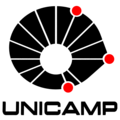
\includegraphics[width=0.2\textwidth]{Figuras/logounicamp}}
    \caption{Legenda}   \label{fig:museo:fig}           
\end{figure}
\begin{itemize}
	\item IMECC
	\item EnCPos
	\item Unicamp
	\end{itemize}
Referenciar Figura \ref{fig:museo:fig}.
\end{frame}	

\subsubsection{ }


%========================================================
\begin{frame}{Patrocínio}  %
%========================================================

\begin{figure}[ht]
   \centering
   %%----primera subfigura----
   \subfloat[texto fig4]{\label{fig:museo:fig4}         %% Etiqueta para la primera subfigura
        
\includegraphics[width=0.3\textwidth]{Figuras/LogoLINEAR}}
  \hspace{0.1\linewidth}
   %%----segunda subfigura----
   \subfloat[texto fig5]{\label{fig:museo:fig5}         %% Etiqueta para la segunda subfigura
        \includegraphics[width=0.3\textwidth]{Figuras/logoUNISOMA}}
\end{figure}
	\begin{itemize}
	\item Linear Softwares Matemáticos: Figura \ref{fig:museo:fig4}.
	\item Unisoma: Figura \ref{fig:museo:fig5}
	\end{itemize}
\end{frame}	
%========================================================
\section{Seção 2}
%========================================================
\begin{frame}{Equações}
%========================================================

\begin{equation*} 
\begin{cases}
 \dfrac{\partial W}{\partial t}	+	(W\cdot \nabla )W =-\dfrac{ 1}{\rho}\nabla p +
			 \dfrac{ \mu}{\rho}\nabla^2 W =0\\
\\
\nabla \cdot W =0
\end{cases}
\end{equation*}
Onde: 
\end{frame}
%==========================================
%==========================================
\begin{frame}
\begin{equation*} 
\text{Momento x:} \hspace{1cm} 
\rho \Big(	 \frac{w_1 \partial w_1}{\partial x}	+	\frac{ w_2\partial w_1}{\partial y}		\Big) -
\mu	 \Big(	 \frac{\partial^2w_1}{\partial x^2}	+	\frac{\partial^2w_1}{\partial y^2}	\Big) +
			 \frac{\partial P}{ \partial x} =0
\end{equation*}
\begin{equation*} 
\text{Momento y:} \hspace{1cm} 
\rho \Big(	 \frac{w_1 \partial w_2}{\partial x}	+	\frac{ w_2\partial w_2}{\partial y}		\Big) -
\mu	 \Big(	 \frac{\partial^2w_2}{\partial x^2}	+	\frac{\partial^2w_2}{\partial y^2}	\Big) +
			 \frac{\partial P}{ \partial y} =0
\end{equation*}
\begin{equation} \label{eq:cont}
\text{Continuidade:} \hspace{1cm} 
	 \frac{\partial w_1}{\partial x}	+	\frac{ \partial w_2}{\partial y}		 =0	\hspace{4.2cm}
\end{equation}
Referenciar \ref{eq:cont}
\end{frame}
%=============================
%=============================================
\section{Parâmetros}
%=============================================
\begin{frame}{Parâmetros}
\begin{table}[H]
\centering
\begin{tabular}{|c|c|c|c|}
\hline \hline
	Parâmetros 	& 		$E_1$ 		& $E_2$		& 	Unidades 		\\
\hline \hline
	$\alpha$ 	& 	$10^{-3}$ 		& 	$10^{-3}$ 	& 	$km^2/h$		\\
\hline
	$u$ 		& 	$-4\times 10^{-3}$	& 	$10^{-5}$&		$km/h$		\\
\hline
	$v$ 		& 	$-4\times 10^{-3}$	& 	$10^{-5}$& 	$km/h$			\\
\hline
	$\mu$ 	& 		0.05 	& 		0.035 			& 	$h^{-1}$		\\
\hline
	$\lambda$ & 		0.03 	& 	0.04 				& 	$h^{-1}$		\\
\hline
	$\kappa$ 	&	 	20		& 20		& $n^0 \; individuos/ua$\\
\hline \hline
\end{tabular}
\caption{Parâmetros.} \label{tab:tabela_p}
\end{table}
Referenciar Tabela \ref{tab:tabela_p}
\end{frame}

\section{Referências}

\bibliographystyle{abbrv}
\bibliography{Bibliografia.bib}


% - - - - - - - - - - - - - - - - - - - - - - - - - - - - - - - - - - - - - - - - - - - - - - - - - - - - - - - -
%\frame{ \frametitle{Principais Refer\^encias }

%\begin{enumerate}
%  \item
%  \item 
%\end{enumerate}
%}
%\emd{frame}
\end{document}

